\chapter{Background} \label{chap:Introduction}

An article, published in 2018 by David Main in the Atlantic, asserts that "Glass has changed the world like no other substance" despite often being taken for granted \nolinebreak \cite{Main}. Main does an excellent job delving into the history behind human adaptation of glass, from prehistoric times when volcanic glasses were used as tools, to its likely initial manufacture and its spread throughout Mesopotamia more than four millennia ago, followed by the development of glass blowing, which arose in first-century Jerusalem, and the appearance of clear glass allowing for more functional, rather than solely ornamental, implementations.  While many materials have significantly impacted technological and cultural development, glass ranks among the most influential—comparable to metal alloys, petrochemicals, and in recent times, semiconductors.  In the sections that follow, we will first define what constitutes a glass and explore the structural and dynamic characteristics that distinguish glasses from other states of matter.

In modern times, an astonishing variety of glasses are manufactured on an industrial scale. Particularly notable are silicate-based glasses, which can be doped with diverse substances—such as lead, germanium oxide, zirconium, titanium, or barium—to precisely control their refractive index. Adjusting the refractive index has both ornamental and practical applications. For instance, lead oxide increases optical dispersion, enhancing the visual aesthetics of decorative glass, while in fiber-optic cables, doping allows higher flexibility and reduced optical leakage by manipulating the critical angle of internal reflection \nolinebreak \cite{Grattan,Jiang}.  

Beyond optical properties, glasses can also be engineered for specific thermal or mechanical characteristics. Boron trioxide doping, for example, is frequently used to reduce thermal expansion, while aluminum oxide can enhance tensile strength and heat capacity. \nolinebreak \cite{Ashby,Askeland}.  Such tailored glasses have profound implications for practical applications like waste disposal. A particularly promising application involves using glass matrices for immobilizing nuclear waste, dramatically reducing risks of contamination by preventing waste materials from leaching into groundwater. \nolinebreak \cite{Plodinec,Ojovan2011}.

The classification of glass extends well beyond simple silicate systems. Amorphous metallic alloys, often referred to as metallic glasses, have been extensively researched since their discovery roughly half a century ago due to their unique mechanical strength and magnetic characteristics \nolinebreak \cite{Greer1947,Ashby}.  Spin glasses represent another important class of non-silicate glasses, characterized by their magnetic domains undergoing transitions analogous to structural glass transitions—making them intriguing subjects of study since the mid-1970s \nolinebreak \cite{RevModPhys.58.801,Mydosh,PhysRevLett.35.1792}.

Water serves as an intriguing example of a substance that forms a glass only under exceptional conditions. Its high heat capacity and strong hydrogen-bond network typically allow crystallization to outpace vitrification. Thus, forming glassy water requires rapid cooling to its glass transition temperature, around $137~\si{\kelvin}$, on a millisecond timescale. However, glassy water has been produced under laboratory conditions and is found to exhibit unusual characteristics, including a tendency to transition directly from a glassy state into a crystalline state upon heating \nolinebreak \cite{Angell2}. Glassy water has also been found, predominantly \via neutron scattering experiments, to exhibit long-range structural order while lacking local order—an atypical feature for a glass, as will be discussed in \sect \nolinebreak \ref{sec:sctructualdesc} \nolinebreak \cite{Martelli,Bradley}.  

It is, perhaps, strange to think of water as being a glass, yet evidently it can be and exhibits remarkable properties when in a glassy state. As unusual a material as it is, glassy water is not solely relegated to laboratory experiments. Water in the Kuiper belt has slowly nucleated over billions of years to form comets and other celestial bodies. This nucleation occurs so slowly, and at such low temperatures, that individual molecules lack sufficient mobility to reorient into a crystalline structure, thus forming, one monolayer at a time, an amorphous glassy ice. A marvelous article on the topic of glassy water, published in \emph{Physics Today}, asserts that “glassy water may be the most common form of water in the universe” \nolinebreak \cite{Debenedetti2}. Indeed, water is among the most abundant molecular species in the universe, second only to molecular hydrogen in many astrophysical environments; consequently, amorphous (glassy) water is likely the most common glass in the universe \cite{Herbst2009,Fraser2001}.

This is not the only instance of atypical behavior. The melting point of water exhibits a negative slope above the triple point due to its unusual lattice structure, resulting in expansion upon freezing. Even at low temperatures, crystalline ice can undergo significant structural transformations under compression. Near the melting line (down to approximately $-25\,^{\circ}\mathrm{C}$), increasing pressure can induce melting due to the negative slope of the ice--liquid coexistence curve. At lower temperatures, however, compression no longer produces a liquid phase but instead drives transitions to other crystalline polymorphs or to amorphous ice. In particular, the pressure-induced amorphization of ice Ih, first observed by Mishima \etal in the mid-1980s \cite{Mishima}, represents a collapse of the crystalline lattice into a disordered solid rather than true melting. Here, a glass is formed \via pressure-induced amorphization well below the glass transition temperature. In this instance, amorphization depends on the mechanical instability of the open crystalline lattice under compression rather than on melting into a liquid phase.

However, pressure-induced amorphization has also been observed in crystalline silica, a more typical glass-forming system, as well as in the SiO$_2$ analog GeO$_2$ \nolinebreak \cite{Hemley,Wolf}. More broadly, pressure-induced amorphization (PIA) has now been reported in scores of materials spanning network oxides, molecular solids, and organic systems. While relatively open-network structures are a common motif among systems exhibiting PIA, they are not a strict requirement. For example, benzene undergoes PIA when sufficiently high pressures disrupt its ring structure, forming amorphous hydrocarbon configurations. More recently, pressure-induced charge amorphization has been reported in materials such as BiNiO$_3$, wherein the lattice remains crystalline while the electronic degrees of freedom become glassy. These diverse examples illustrate that PIA represents amorphization from an initially crystalline state under applied pressure and may arise through multiple structural or electronic mechanisms depending on how pressure reshapes the underlying energy landscape \nolinebreak \cite{Ponyatovsky}.  

There also exist countless organic substances that readily form amorphous glassy solids that permeate the literature.  They find applications in medicine, for example the use of glassy scaffolds for drug delivery or even potentially taking advantage of the glassy state of a drug itself where the lower Gibbs energy associated with increased structural entropy may give rise to greater water solubility and thus increase the efficacy of delivery \nolinebreak \cite{Chidambaram,Krynski}.  Polymethyl methacrylate (PMMA), a strong thermoplastic often referred to as an acrylic glass and marketed under the brand names Plexiglass, Acrylite, and Lucite among others, has found a wide variety of applications since its invention by Dupont in the early 1930's including automobile manufacture,  aircraft windows, marker boards, and even the ceiling of the Houston Astrodome ballpark due to its high transparency, resistance to external elements such as UV light and water, and other beneficial properties \nolinebreak \cite{Lucite}.  Polylactic acid (PLA) is another glass-forming organic thermoplastic which has found extensive application in rapid prototyping due to the ability of such materials to be softened in a controlled manner upon heating \nolinebreak \cite{Sodergard}.  Metallic glasses also share this characteristic and thus are quickly capturing interest for their potential to allow for direct 3D printing of metallic parts \nolinebreak \cite{MetallicGlass}.  

The material qualities that define a glass are still somewhat contested today, however functional definitions do exist and will be the topic of the following section.  Here it may suffice to say that the term glass describes a vast array of materials spanning countless applications from window panes to, perhaps somewhat surprisingly, even cotton candy\textemdash a sucrose glass \nolinebreak \cite{Hartel2014candy}.  In 2015 the Carnegie Science Center of Pittsburgh had a marvelous display spotlighting the indispensable role that glasses play in our day-to-day lives. It was somewhat disappointing to me that a prominent display case labeled "Is it Glass" did not contain any cotton candy\textemdash arguably almost as disappointing as the fact that such a fascinating topic as to what constitutes a glass, so poorly understood by the public, was relegated to a small non-imposing display case. 
\graphicspath{{Chapters/Background/Figures/}}
\begin{figure} [!htbp]
	\centering
	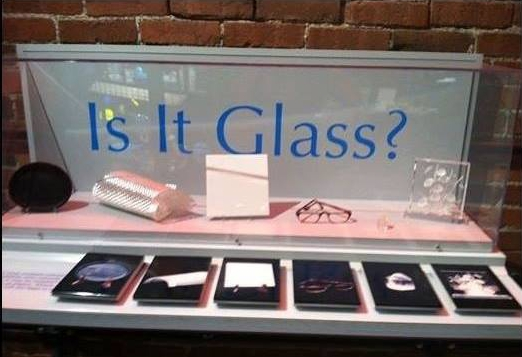
\includegraphics[width=.8\linewidth] {CarnegieGlass.jpg}
	\caption{Exhibit on display at the Carnegie Science Center (2015)}
	\label{figure:IsitGlass}
\end{figure} 

Sucrose, or common sugar, is in fact an excellent glass-forming material despite typically being encountered in its crystalline form. A familiar example of a sucrose glass—one that for many evokes childhood memory—is peanut brittle. During its preparation a mixture of sugar, corn syrup, and water is heated well above the boiling point of pure water. As boiling proceeds, water is progressively removed and the composition continuously evolves. Because water acts as a strong plasticizer for sucrose, its removal causes the glass transition temperature $T_g$ of the mixture to rise steadily throughout the cooking process.

At early stages, when the water content remains high, pulling filaments from the syrup produces strings that readily flow and collapse back into the pot. If cooled to room temperature at this stage, the mixture would form a viscous liquid rather than a glass, as its $T_g$ lies well below ambient temperature. As evaporation continues, viscosity increases dramatically and the glass transition temperature approaches room temperature. When thin filaments drawn from the pot rapidly stiffen and snap, this indicates that the evolving composition has reached a state for which cooling to ambient conditions will carry the system below its glass transition temperature. 

Thus, the critical transformation in peanut brittle is not simply cooling through $T_g$, but rather the continuous elevation of $T_g$ through removal of the plasticizing water. Pulling the syrup provides a practical means of gauging the evolving composition and determining when the material, upon cooling, will vitrify into a rigid glass rather than remain rubbery or viscous.

If you have never seen peanut brittle made, set this dissertation down for a spell and go make a batch, for in the sections that follow, we will be delving into the details of what constitutes a glass as well as the molecular dynamics of the transition from a liquid to a glassy state.  As is the case with all dissertations, beyond this introduction the material will become less colloquial and more technical.  Having a plate of peanut brittle to enjoy as you read could certainly do no harm and may even serve to bestow on you a certain experiential intuition regarding the glass transition process.  Besides, as Pamela Travers would almost certainly assert, "A glass made of sugar helps the medicine go down \nolinebreak \cite{Travers}."
	 

\section{Glasses and Glass-Forming Liquids}

Before one can have a meaningful discussion of glassy dynamics and the glass transition, one must define what constitutes a glass.  Zarzycki offers two potential definitions of glass\textemdash one operational and the other structural \nolinebreak \cite{Zarzycki}.  From an operational standpoint, one might define a glass as a liquid rapidly thermally quenched into a non-crystalline solid phase. Alternatively, from a structural perspective, a glass may be defined more generally simply as a non-crystalline solid\textemdash ignoring the means by which this state was obtained.  As Zarzycki delineates, both of these definitions fall short of providing a sufficient description of the glassy state. The simple structural perspective is too broad, encompassing materials such as gels that do not share the physical attributes of a glass. Conversely, his operational definition is too specific, omitting states that are structurally identical yet were arrived at \via means other than thermal quenching. 

Such alternative pathways include compression, which will be central to the topics of \chap \nolinebreak \ref{chap:Glycerol} and \nolinebreak \ref{chap:PCS}; pressure-induced amorphization as demonstrated by Mishima or Hemley \etal \nolinebreak \cite{Hemley,Mishima}; and cold deposition, as previously discussed regarding water ice on comets formed \via accretion \nolinebreak \cite{Debenedetti2}.  His conclusion, and the general consensus today, is that the solution lies in a definition of the glassy state which incorporates the structural perspective with the added caveat that glasses constitute a non-equilibrium solid-state system\textemdash a merger of structural and dynamic descriptions.  We will begin by examining the structural description of glasses and then proceed to consider their dynamic characteristics in detail.

\subsection{Structural Description}\label{sec:sctructualdesc}

Zarzycki's definition still requires further clarification.  Is a glass a liquid, solid, or a separate phase of matter in its own right?  One may be tempted to assert that glass is nothing more than a highly viscous liquid whose viscosity may be rapidly diverging however will still flow\textemdash albeit on a remarkably long timescale.  Indeed, one would not be hard pressed to find, even among physicists, those who believe that cathedral stained glass is thicker at the bottom of the pane due to the glass having flowed over the centuries under the influence of gravity\textemdash a very common misconception. In reality, medieval glaziers commonly installed panes with the thicker edge at the bottom for structural stability, reflecting the manufacturing process rather than viscous flow. The best models of molecular dynamics in glassy systems must be heavily extrapolated to address such timescales; nevertheless, even extremely conservative estimates place the average timescale required for these silicate glasses to flow appreciably at ambient temperatures several orders of magnitude beyond the age of the Universe \nolinebreak \cite{Zanotto}. 

In light of this, to assert that a material in a glassy state is `fluid' in any colloquial sense may seem absurd. However, one's incredulity does not a valid definition make, and one cannot dismiss the fact that a glass's radial distribution function is often indistinguishable from that of the liquid state as conceptually illustrated in \fig \nolinebreak \ref{GlassCorrComp}.

The radial distribution function, alternatively referred to as the pairwise correlation function, is a quantity defined as the expectation value of the particulate number density in a region as a function of distance from an origin placed at any arbitrarily representative particle or molecule within a bulk volume of material.  This is best conceptualized as the ensemble average of the distance between all other particles or molecules as measured from each individual particle or molecule within a bulk material.

\begin{figure}[!htbp]
	\centering
	\begin{minipage}[t]{.29\textwidth}
		\centering
		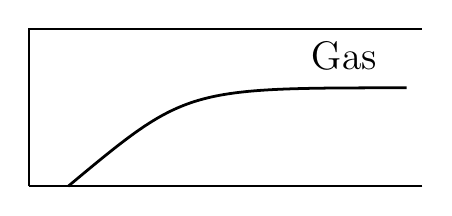
\begin{tikzpicture}	
		%Frame for plot of Gas
		\draw[thick] (0,0.25)--(0,2.25)--(5,2.25); 
		\draw[thick] (5,.25)--(0,.25);
		\draw[line width=1pt] (.5,.25) .. controls (2,1.5) .. (4.8,1.5);
		\node[] at (4,1.9) {\Large Gas};
		\end{tikzpicture}
	\end{minipage}
	\begin{minipage}[t]{.1666\textwidth}
		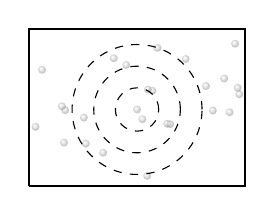
\begin{tikzpicture}	
		%Random Locations for Gas
		\foreach \y in {1,2,3,4,5}
		\foreach \x in {1,2,3,4,5}
		\shade[ball color = gray!40, opacity = 0.4] (1.325*rand+1.375,.95*rand+1.25) circle (.05cm);
		\shade[ball color = gray!40, opacity = 0.4] (1.375,1.225) circle (.05cm);
		\draw[thick] (0,0.25)--(0,2.25)--(2.75,2.25)--(2.75,.25)--(0,.25);
		\draw[dashed] (1.375,1.225) circle (.275cm);	
		\draw[dashed] (1.375,1.225) circle (.55cm);
		\draw[dashed] (1.375,1.225) circle (.825cm);		
		\end{tikzpicture}
	\end{minipage}
	\begin{minipage}[t]{.29\textwidth}
		\centering
		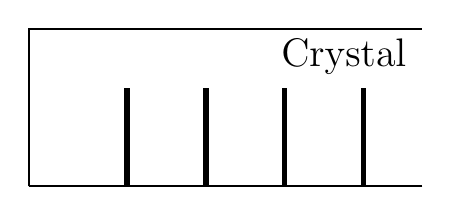
\begin{tikzpicture}	
		%Frame for plot of Crystal
		\foreach \x in {0,1,2,3}
		\draw[line width=2pt] (\x+1.25,.25)--(\x+1.25,1.5);
		\draw[thick] (0,0.25)--(0,2.25)--(5,2.25); 
		\draw[thick] (0,0.25)--(0,2.25)--(5,2.25);
		\draw[thick] (5,.25)--(0,.25);
		\node[] at (4,1.9) {\Large Crystal};
		\end{tikzpicture}
	\end{minipage}
	\begin{minipage}[t]{.1666\textwidth}
		\centering
		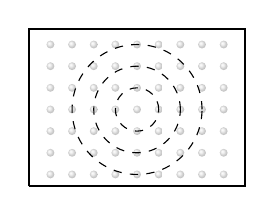
\begin{tikzpicture}	
		%Random Locations for Crystal
		\foreach \y in {1,2,3,4,5,6,7}
		\foreach \x in {1,2,3,4,5,6,7,8,9}
		\shade[ball color = gray!40, opacity = 0.4] (.275*\x,.275*\y+.125) circle (.05cm);
		\draw[thick] (0,0.25)--(0,2.25)--(2.75,2.25)--(2.75,.25)--(0,.25);
		\draw[dashed] (1.375,1.225) circle (.275cm);	
		\draw[dashed] (1.375,1.225) circle (.55cm);
		\draw[dashed] (1.375,1.225) circle (.825cm);			
		\end{tikzpicture}
	\end{minipage}
	\begin{minipage}[t]{.29\textwidth}
		\centering
		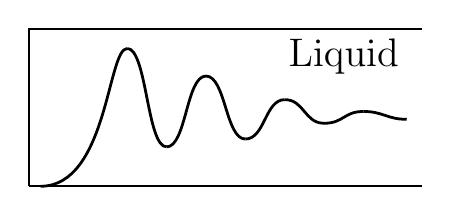
\begin{tikzpicture}	
		%Frame for plot of Liquid
		\draw[thick] (0,0.25)--(0,2.25)--(5,2.25); 
		\draw[thick] (5,.25)--(0,.25);
		\draw[line width=1pt] (.15,.25) .. controls (1,.25) and (1,2) .. (1.25,2) ;
		\draw[line width=1pt] (1.25,2) .. controls (1.5,2) and (1.5,.75) .. (1.75,.75);
		\draw[line width=1pt] (1.75,.75) .. controls (2,.75) and (2,1.65) .. (2.25,1.65) ;
		\draw[line width=1pt] (2.25,1.65) .. controls (2.5,1.65) and (2.5,.85) .. (2.75,.85) ;
		\draw[line width=1pt] (2.75,.85) .. controls (3,.85) and (3,1.35) .. (3.25,1.35) ;
		\draw[line width=1pt] (3.25,1.35) .. controls (3.5,1.35) and (3.5,1.05) .. (3.75,1.05) ;
		\draw[line width=1pt] (3.75,1.05) .. controls (4,1.05) and (4,1.2) .. (4.25,1.2) ;
		\draw[line width=1pt] (4.25,1.2) .. controls (4.5,1.2) and (4.55,1.1) .. (4.8,1.1) ;
		\node[] at (4,1.9) {\Large Liquid};
		\end{tikzpicture}
	\end{minipage}
	\begin{minipage}[t]{.1666\textwidth}
		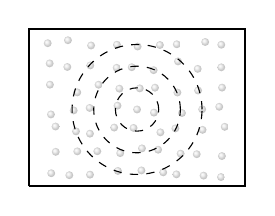
\begin{tikzpicture}	
		%Random Locations for Liquid
		\foreach \y in {1,2,3,4,5,6,7}
		\foreach \x in {1,2,3,4,6,7,8,9}
		\shade[ball color = gray!40, opacity = 0.4] (.275*\x+.275*rand/4,.275*\y+.275*rand/4+.125) circle (.05cm);
		\foreach \y in {1,2,3,5,6,7}
		\shade[ball color = gray!40, opacity = 0.4] (1.375+.275*rand/4,.275*\y+.275*rand/4+.125) circle (.05cm);	
		\shade[ball color = gray!40, opacity = 0.4] (1.375,1.225) circle (.05cm);		
		\draw[thick] (0,0.25)--(0,2.25)--(2.75,2.25)--(2.75,.25)--(0,.25);
		\draw[dashed] (1.375,1.225) circle (.275cm);	
		\draw[dashed] (1.375,1.225) circle (.55cm);
		\draw[dashed] (1.375,1.225) circle (.825cm);		
		\end{tikzpicture}
	\end{minipage}
	\begin{minipage}[t]{.29\textwidth}
		\centering
		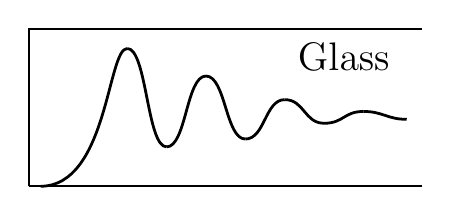
\begin{tikzpicture}	
		%Frame for plot of Gass
		\draw[thick] (0,0.25)--(0,2.25)--(5,2.25); 
		\draw[thick] (5,.25)--(0,.25);
		\draw[thick] (0,0.25)--(0,2.25)--(5,2.25); 
		\draw[thick] (5,.25)--(0,.25);
		\draw[line width=1pt] (.15,.25) .. controls (1,.25) and (1,2) .. (1.25,2) ;
		\draw[line width=1pt] (1.25,2) .. controls (1.5,2) and (1.5,.75) .. (1.75,.75);
		\draw[line width=1pt] (1.75,.75) .. controls (2,.75) and (2,1.65) .. (2.25,1.65) ;
		\draw[line width=1pt] (2.25,1.65) .. controls (2.5,1.65) and (2.5,.85) .. (2.75,.85) ;
		\draw[line width=1pt] (2.75,.85) .. controls (3,.85) and (3,1.35) .. (3.25,1.35) ;
		\draw[line width=1pt] (3.25,1.35) .. controls (3.5,1.35) and (3.5,1.05) .. (3.75,1.05) ;
		\draw[line width=1pt] (3.75,1.05) .. controls (4,1.05) and (4,1.2) .. (4.25,1.2) ;
		\draw[line width=1pt] (4.25,1.2) .. controls (4.5,1.2) and (4.55,1.1) .. (4.8,1.1) ;
		\node[] at (4,1.9) {\Large Glass};
		\end{tikzpicture}
	\end{minipage}
	\begin{minipage}[t]{.1666\textwidth}
		\centering
		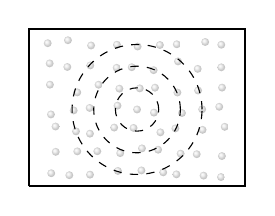
\begin{tikzpicture}	
		%Random Locations for Glass
		\foreach \y in {1,2,3,4,5,6,7}
		\foreach \x in {1,2,3,4,6,7,8,9}
		\shade[ball color = gray!40, opacity = 0.4] (.275*\x+.275*rand/4,.275*\y+.275*rand/4+.125) circle (.05cm);
		\foreach \y in {1,2,3,5,6,7}
		\shade[ball color = gray!40, opacity = 0.4] (1.375+.275*rand/4,.275*\y+.275*rand/4+.125) circle (.05cm);	
		\shade[ball color = gray!40, opacity = 0.4] (1.375,1.225) circle (.05cm);		
		\draw[thick] (0,0.25)--(0,2.25)--(2.75,2.25)--(2.75,.25)--(0,.25);
		\draw[dashed] (1.375,1.225) circle (.275cm);	
		\draw[dashed] (1.375,1.225) circle (.55cm);
		\draw[dashed] (1.375,1.225) circle (.825cm);		
		\end{tikzpicture}
	\end{minipage}
	\caption{Typical radial correlation functions for a gas, liquid, glass, and crystal.  This figure is derivative of that originally published by Johari. \cite{Johari}} \label{GlassCorrComp} 
\end{figure}

Significantly simplified two-dimensional representations of radial distribution functions and the structures giving rise to them for a gas, liquid, crystal, and glass are provided in the aforementioned \fig \nolinebreak \ref{GlassCorrComp}.  Note that the exact particle locations for this figure were determined implementing a random number generator and thus are not representative of the ensemble average resulting from any specific intermolecular potential.  This figure is relevant to a discussion of the characteristics typical of pairwise correlation functions for these four material states only in the most general of terms.  The two-dimensional analog of a crystalline structure is shown in greater detail here in \fig \nolinebreak \ref{distributionDefined} where the characteristic radii between horizontally and vertically adjacent particles are labeled $r_1$.  The characteristic radii corresponding to the nearest neighbor, next nearest neighbor, and next-next nearest neighbor are labeled $r_1$, $r_2$ and $r_3$ respectively.  These will exhibit rapidly decreasing correlation amplitudes for higher order nearest neighbors.  The corresponding radial distribution function exhibits very sharp periodic peaks associated with these infinitely repeating lattice spacings.  The exact appearance of a radial distribution function for any real crystalline bulk material can clearly be quite complex and will vary from one material to the next as it depends directly upon the crystal symmetry, however it will always consist of such well defined periodic peaks.  The arguably oversimplified crystalline pair correlation spectra shown in \fig \nolinebreak \ref{GlassCorrComp} ignores all peaks associated with these off diagonal contributions from the lattice structure to provide an even further conceptually idealized spectra.  Strictly speaking, such a simple correlation spectra could only ever arise from a one dimensional distribution of evenly spaced particles however it represents the behavior of a repetitive lattice structure sufficiently well for the purposes of this discussion, and in fact it is not uncommon for solid-state physics texts to similarly describe the band structure along a single direction of a 3D crystalline structure.

\begin{figure} [!htbp]
	\centering
	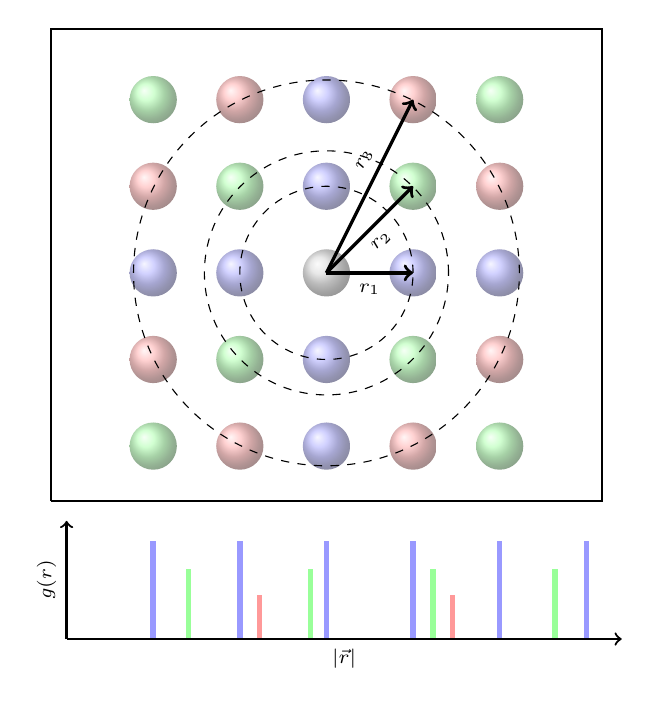
\begin{tikzpicture}	
	%Top Row of Particles
	\foreach \x in {3,7}
	\shade[ball color = green!40, opacity = 0.6] (1.1*\x,1.1*6+.5) circle (.3cm);
	\foreach \x in {4,6}
	\shade[ball color = red!40, opacity = 0.6] (1.1*\x,1.1*6+.5) circle (.3cm);
	\shade[ball color = blue!40, opacity = 0.6] (1.1*5,1.1*6+.5) circle (.3cm);
	
	%2nd Row of Particles
	\foreach \x in {3,7}
	\shade[ball color = red!40, opacity = 0.6] (1.1*\x,1.1*5+.5) circle (.3cm);
	\foreach \x in {4,6}
	\shade[ball color = green!40, opacity = 0.6] (1.1*\x,1.1*5+.5) circle (.3cm);
	\foreach \x in {5}
	\shade[ball color = blue!40, opacity = 0.6] (1.1*\x,1.1*5+.5) circle (.3cm);
	
	%3rd Row of Particles
	\foreach \x in {3,4,6,7}
	\shade[ball color = blue!40, opacity = 0.6] (1.1*\x,1.1*4+.5) circle (.3cm);
	
	%4th Row of Particles
	\foreach \x in {3,7}
	\shade[ball color = red!40, opacity = 0.6] (1.1*\x,1.1*3+.5) circle (.3cm);
	\foreach \x in {4,6}
	\shade[ball color = green!40, opacity = 0.6] (1.1*\x,1.1*3+.5) circle (.3cm);
	\foreach \x in {5}
	\shade[ball color = blue!40, opacity = 0.6] (1.1*\x,1.1*3+.5) circle (.3cm);
	
	%Bottom Row of Particles
	\foreach \x in {3,7}
	\shade[ball color = green!40, opacity = 0.6] (1.1*\x,1.1*2+.5) circle (.3cm);
	\foreach \x in {4,6}
	\shade[ball color = red!40, opacity = 0.6] (1.1*\x,1.1*2+.5) circle (.3cm);
	\foreach \x in {5}
	\shade[ball color = blue!40, opacity = 0.6] (1.1*\x,1.1*2+.5) circle (.3cm);
	
	%Central Ball in Red
	\shade[ball color = gray!40, opacity = 0.6] (1.1*5,1.1*4+.5) circle (.3cm);
	
	%Outline
	\draw[thick] (2,2)--(2,8)--(9,8)--(9,2)--(2,2);
	\draw[dashed] (5.5,4.9) circle (1.1cm);		
	\draw[dashed] (5.5,4.9) circle (1.55cm);	
	\draw[dashed] (5.5,4.9) circle (2.45cm);	
	\draw[->,very thick,black] (5.5,4.9)--(6.6,4.9) node[draw=none,fill=none,font=\scriptsize,midway,below] {$r_1$};
	\draw[->,very thick,black] (5.5,4.9)--(6.6,1.1*5+.5) node[draw=none,fill=none,font=\scriptsize,midway,below,rotate =45] {$r_2$};
	\draw[->,very thick,black] (5.5,4.9)--(6.6,1.1*6+.5)
	node[draw=none,fill=none,font=\scriptsize,anchor=south west,midway,rotate =63.435] {$r_3$};
	
	
	%Primary Peaks
	\foreach \x in {1,2,3,4,5,6}
	\draw[line width=2pt,color = blue!40] (2.2+\x*1.1,.25)--(2.2+\x*1.1,1.5);
	%First Harmonic
	\foreach \x in {1,2,3,4}
	\draw[line width=2pt,color = green!40] (2.2+\x*1.55,.25)--(2.2+\x*1.55,1.13388);
	%Third Harmonic
	\foreach \x in {1,2}
	\draw[line width=2pt,color = red!40] (2.2+\x*2.45,.25)--(2.2+\x*2.45,.809);
	%Radial Distribution Function
	\draw[->,thick] (2.2,0.25)--(9.25,.25) node[draw=none,fill=none,font=\scriptsize,midway,below,rotate =0] {$\left | \vec{r} \right |$};; 
	\draw [->,thick] (2.2,0.25) -- (2.2,1.75) node[draw=none,fill=none,font=\scriptsize,midway,above,rotate =90] {$g(r)$};
	
	
	\end{tikzpicture}  \caption{A crystalline solid exhibits one or more characteristic radii, for which adjacent individual particles or molecules appear at integer multiples.  The corresponding radial distribution function for such a material will consist of sharp periodic peaks.} \label{distributionDefined} 
\end{figure} 

Conversely, gases exhibit no such periodic order.  Due to the strong yet exceedingly short range Coulombic repulsion, molecules will spend very little time in extremely close proximity, existing mostly in a free state where intermolecular interactions are negligible.  As such, their pairwise correlation function will very rapidly approach a uniform value corresponding to the average particle density.  An idealized representation of this is provided in the top left window of \fig \nolinebreak \ref{GlassCorrComp}.

From a structural perspective, both liquids and glasses will exhibit radial distributions functions that appear almost as if they consisted of a damped superposition of the gas and crystalline states.  This arises due to the fact that the intermolecular interactions between the constituent molecules of both liquids and glasses are not negligible.  Short-range order emerges as bonds between adjacent constituent molecules are formed.  As this order is at the same time imperfect relative to the crystalline structure, short range, and in the case of a liquid also of short duration, it will manifest itself in the broadening and dampening of the periodic peaks of the corresponding pairwise correlation function.  Representative idealized liquid and glass radial distribution functions are provided in \fig \nolinebreak \ref{GlassCorrComp} as well.  Note the periodic peaks that correspond to an imperfect crystalline structure in short order giving way to an utter lack of long range order indicative of a gas\textemdash albeit at significantly higher density.  

Similarities between the radial correlation functions for a liquid and a glass are worthy of note. Structurally, they are nearly\textemdash if not entirely\textemdash identical. However, they differ vastly in their dynamics. For a liquid, the radial correlation function can be thought of either as arising from a time average of the molecular positions or, equivalently, from an ensemble average calculated from the positions of all individual particles at a single instant in time. Conversely, the dynamics of a glass—being an amorphous solid—are such that its radial correlation function is best understood solely in terms of an ensemble average, since constituent molecules do not move appreciably on experimentally meaningful timescales. Thus, we encounter the curious condition of two material states possessing identical structure yet fundamentally different dynamics. Having explored the structural similarities and differences between glasses and liquids, we now turn our attention to their dynamic properties, particularly how these dynamics reflect differences in molecular motion and energy landscapes.

\subsection{Dynamic Description}

Molecules in a gas state have high enough energy on average that they do not really "feel" the potential energy landscape produced by their neighbors.  They take on a relatively random and highly degenerate spatial distribution where intermolecular interactions are limited to the strong yet exceedingly short range Coulombic repulsion of their electronic shells.  Thus the pairwise correlation function for a well thermalized gas will exhibit very little structure beyond a rapid increase in correlation, arising from this Coulombic repulsion repelling other molecules at close proximity, quickly leveling off to a region of constant number density, beyond the influence of this repulsive force, that will extend indefinitely as demonstrated in \fig \nolinebreak \ref{GlassCorrComp}.

Gases and crystals are, in this sense, polar opposite scenarios in that the former has sufficient thermal energy that the potential landscape arising from the intermolecular forces is almost irrelevant as molecules spend very little time in close enough proximity to any other molecule for even the dominant Coulombic interaction to play a major role in their dynamics, yet the latter has sufficiently low thermal energy such that dynamics are dominated by intermolecular forces beyond Coulombic repulsion\textemdash higher order terms such as dipole or other types of interactions depending on the nature of the constituent atoms making up the crystal.  Molecules in a crystalline state certainly \textit{feel} their potential energy landscape, yet are not free to explore it as most of that parameter space is energetically inaccessible. Thus they are locked into discrete, highly symmetric arrangements associated with the lowest energy structural state of the bulk system. These are the two extremes of which the liquid state is an intermediate.  

Within the energetically intermediate liquid state, molecules or particles have sufficient energy to explore their potential energy landscape yet still be heavily influenced, and to some extent confined, by said landscape.  Short lived bonds between molecules form, increasing the average time in which they are in close proximity and giving rise to cooperative motion.  However these nearest neighbor bonds \textit{are} very short lived\textemdash the activation energy required to break the bonds being on the order of the thermal energy, $k_BT$, of the material. The bonds conforming to the lowest energy orientations corresponding to the crystalline structure, though not exclusively occurring, will clearly be statistically favored.  Thus liquids exhibit the rapid emergence, and subsequent disintegration, of short-range order that may be described as spatially distorted crystalline arrangements.  One would expect that the radial distribution function of a liquid will therefore exhibit structures that resemble the crystalline peaks over a short range, though broadened due to thermal motion and the absence of long-range positional order. However, over sufficiently large separations, these short-lived local nucleations bear no correlation from one region to the next and, as such, the radial correlation function for a liquid approaches unity at large radii\textemdash reflecting the absence of long-range order while maintaining the characteristic number density of the liquid phase. The radial correlation function for a liquid displayed in \fig \nolinebreak \ref{GlassCorrComp} shows what would be expected for a state that is intermediate between a gas and a crystalline solid, \ie, broadened crystalline peaks at short range that quickly wash out to a uniform average number density at larger radii.

Another way to describe the liquid state of a glass-forming system, beyond purely energetic considerations, is to consider the timescales on which the potential energy landscape is explored by the system\textemdash \ie, its structural relaxation time. It should be noted that a variety of relaxation processes occur in any glassy system, not all of which are directly associated with the bulk structural rearrangement. These include thermal relaxations as well as processes arising from diffusion and orientational dynamics, the complexity of which depends strongly on the internal degrees of freedom available to the constituent molecules. 

Even relatively simple glass formers typically exhibit two broad dynamical regimes: fast $\beta$-relaxations, which generally display relatively little dependence on temperature and pressure, and the $\alpha$ relaxation process, which is highly sensitive to thermodynamic conditions and may vary by thirteen or more orders of magnitude between the high-temperature or low-pressure liquid and the glassy state. The $\alpha$ relaxation is the structural relaxation mode of the system, associated with the cooperative motion of many nearby particles and involving mechanisms such as the breaking of nearest-neighbor cages, molecular reorientation, and diffusive rearrangement. It is this structural $\alpha$ relaxation process that is the focus of this dissertation.

In the following section we will discuss several probes of these relaxation dynamics, including Photon Correlation Spectroscopy in \sect\nolinebreak \ref{sec:PCSintro}.  Time-domain correlation spectra obtained using this technique on glass-forming systems are generalized in \fig \nolinebreak \ref{figure:RelaxationShiftIntro} to illustrate this dynamic behavior under varying thermodynamic conditions.  Here, the correlation time, $\tau$, is simply the average time required for a bulk material to relax having been subjected to some form of mechanical perturbation\textemdash  inherently tied to the imaginary component of the bulk modulus. Generally speaking, the fast $\beta$-relaxation will be relatively unaffected by changing thermodynamic parameters.  However, as the temperature of a liquid decreases or, equivalently, as pressure increases, the $\alpha$ relaxation time increases continuously over many orders of magnitude. In the high-temperature or low-pressure liquid, $\tau_{\alpha}$ is typically on the order of picoseconds, whereas at the glass transition it reaches approximately $10^{2}$ seconds. The rate at which $\tau_{\alpha}$ varies with temperature or pressure depends strongly on the fragility of the liquid, with fragile systems exhibiting especially pronounced changes as $T_g$ is approached, while strong liquids display a more gradual evolution.  Understanding how this structural relaxation time grows as thermal energy is reduced or free volume is diminished under compression is central to describing the nature of the glass transition.

	\pgfplotsset{table/search path={Chapters/Background/Figures},}
\begin{figure}[!htbp]
	\centering
	\begin{tikzpicture} 
		\begin{axis}[
			height=.5\textwidth,
			width=.75\textwidth,
			ylabel={$\left \langle A\left ( 0 \right )A\left ( \tau \right ) \right \rangle$},
			xlabel={Correlation Time ($\tau$)},
			xmin=1E-12, xmax=1E4,
			ymin=0, ymax=1,
			xtick={1E-12,1E-10,1E-8,1E-6,1E-4,1E-2,1E0,1E2,1E4},
			ytick={0.2,0.4,0.6,0.8,1},
			xmode=log,
			ymajorgrids=false,
			grid style=dashed,
			legend style={at={(0.225,.425)}},
			legend image post style={mark=none}
			]
			
			\draw[<-,thick] (1E-11,.9)--(1E-10,.9);
			\node[anchor=west] at (1E-10,.9) {$\beta$-relaxation};
			\draw[->,thick] (5E-8,.6)--(5E-7,.6);
			\node[anchor=east] at (5E-8,.6) {$\alpha$-relaxation};
			\draw[->,very thick] (1E1,.9)--(1E3,.9);
			\node[anchor=south east] at (1E1,.9) {$P \uparrow$};
			\node[anchor=east] at (1E1,.85) {$T \downarrow$};
			
			% Shortest relaxation time (fast liquid)
			\addplot [black, very thick, solid] 
			table [x=time, y=1micro, col sep=comma] {Relaxations.csv};
			\addlegendentry{{\scriptsize 1.00 \;\si{\micro\second}}}
			
			\addplot [black, thick, densely dashed] 
			table [x=time, y=100micro, col sep=comma] {Relaxations.csv};
			\addlegendentry{{\scriptsize 100 \;\si{\micro\second}}}
			
			\addplot [black, semithick, dashed] 
			table [x=time, y=10milli, col sep=comma] {Relaxations.csv};
			\addlegendentry{{\scriptsize 10 \;\si{\milli\second}}}
			
			\addplot [black, semithick, dashdotted] 
			table [x=time, y=1sec, col sep=comma] {Relaxations.csv};
			\addlegendentry{{\scriptsize 1.00 \;\si{\second}}}
			
			% Longest relaxation time (near Tg)
			\addplot [black, dotted] 
			table [x=time, y=100sec, col sep=comma] {Relaxations.csv};
			\addlegendentry{{\scriptsize 100 \;\si{\second}}}
			
		\end{axis} 
	\end{tikzpicture}
	\caption{An idealized set of autocorrelation curves typical of what might be obtained for a glass-forming system. The characteristic structural relaxation time $\tau_\alpha$ falls near the foot of each curve. As temperature is decreased or pressure is increased, the faster $\beta$-relaxation remains relatively fixed; however, the $\alpha$-relaxation shifts to longer times as structural relaxation slows and an increasing fraction of the energy landscape becomes energetically inaccessible.}  
	\label{figure:RelaxationShiftIntro}
\end{figure}

In the most simplistic of terms, glassy materials exhibit the rigidity of a crystalline state, having insufficient thermal energy to readily explore their potential energy landscape, yet maintain the semi-ordered structure of their liquid state.  Their radial correlation functions, as characterized in \fig \nolinebreak \ref{GlassCorrComp}, will be very similar in structure to that of the liquid state, often exhibiting short range crystalline structure albeit with copious irregularities, transitioning into rapidly diminishing structural correlation over longer distances.  A very marked difference between a system in a liquid \vs a glassy state is the apparent violation of ergodicity.  Although the radial correlation function of a glass may be similar to the liquid state in general structure, it may not be quite as identical as implied by \fig \nolinebreak \ref{GlassCorrComp}.  Glassy systems will exhibit mechanical hysteresis stemming from their exceedingly slow structural relaxations. This along with the lower thermal energy of these systems results in intermolecular bonds being much longer lived than in the liquid state which may lead to semi-crystalline domains growing quite large.  Cooperative motion of these domains will play a much greater role in the dynamics of glassy systems than in a liquid state.  These considerations, among others, leave open the question as to whether glass exists as a separate phase of matter or as nothing more than a highly viscous fluid\textemdash a question we will now address.  

\section{The Nature of the Glass Transition}

A material undergoing a change in phase will experience a dramatic and discontinuous shift in bulk properties such as density, specific heat, bulk modulus, thermal expansivity, \etc  Ehrenfest more precisely defined phase transitions as points in the pressure-temperature-volume phase space of the material where discontinuities in the derivatives of the Gibbs free energy with respect to any external thermodynamic parameter emerge.  Transitions between any two states described in \fig \nolinebreak \ref{GlassCorrComp} with the exception of the glass transition will constitute what Ehrenfest described as a first-order phase transition in that it will involve discontinuities in first-order derivatives of the free energy, or equivalently enthalpy, for a transition at constant pressure \nolinebreak \cite{Jaeger}.  The glass transition, however, is distinct from the others in that no such first-order discontinuity exists.  \fig \nolinebreak \ref{figure:Transition} shows the plot of enthalpy or specific volume as a function of temperature for an idealized glass-forming system maintained at constant pressure.  At the freezing temperature, $T_f$, the enthalpy of fusion—equivalently the latent heat of fusion—corresponds to a discontinuous change in enthalpy. Such a discontinuity in the first derivative of the Gibbs free energy is the defining characteristic of a first-order phase transition and is apparent in \fig \nolinebreak \ref{figure:Transition}. In principle, any liquid capable of forming a crystalline structure, if brought to this temperature, provided with a single nucleation point, and allowed to cool slowly enough to maintain thermalization, will form a single-crystal solid that constitutes the global minimum on the potential energy landscape as represented in \fig \nolinebreak \ref{figure:landscape}.  This conceptually idealized projection of the potential energy landscape, adapted from the review by Debenedetti and Stillinger \cite{Debenedetti}, represents the potential energy as a function of a single configurational coordinate. It is, obviously, not possible to aptly describe the potential landscape for any real system graphically as it will span a parameter space whose dimension will be on the order of the number of constituent molecules residing in the bulk multiplied by their individual degrees of freedom.  However this overly simplified single dimensional representation is quite sufficient as a conceptual illustration.  

\begin{figure} [!htbp] 
	\centering
	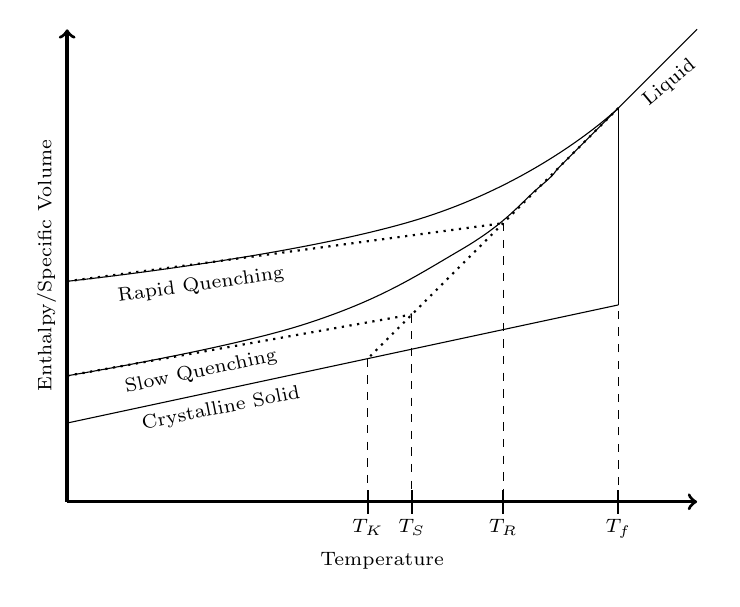
\begin{tikzpicture}
		\draw[very thick,->] (0,0)--(0,6) node[draw=none,fill=none,font=\scriptsize,midway,above,rotate =90] {Enthalpy/Specific Volume};
		\draw[very thick,->] (0,0)--(8,0); \node[draw=none,fill=none,font=\scriptsize] at (4,-.75) {Temperature};
		
		\draw[] (0,1)--(3.81818,1.81818)
		node[draw=none,fill=none,font=\scriptsize,midway,below,rotate = 11.31] {Crystalline Solid};
		\draw[] (3.81818,1.81818)--(7,2.5);
		\draw[] (7,2.5)--(7,5);
		\draw[] (7,5)--(8,6)
		node[draw=none,fill=none,font=\scriptsize,midway,below,rotate = 39.81] {Liquid};
		\draw[dotted, thick] (7,5)--(3.81818,1.81818); 
		
		\draw[thick] (7,-0.15)--(7,0.15);
		\draw[dashed] (7,0)--(7,2.5);
		\node[draw=none,fill=none,font=\scriptsize,below] at (7,-.1) {$T_f$};
		
		\draw  plot[smooth, tension=.7] coordinates {(7,5) (6.75,4.75) (6.5,4.5) (6.25,4.25) (6,4) (5,3.2) (3,2.25) (0,1.6)};
		\node[draw=none,fill=none,font=\scriptsize,rotate = 12] at (1.7,1.65) {Slow Quenching};
		\draw  plot[smooth, tension=.8] coordinates {(7,5) (4.5,3.6) (0,2.8)};
		\node[draw=none,fill=none,font=\scriptsize,rotate = 8] at (1.7,2.75) {Rapid Quenching};
		
		\draw[thick] (5.53846,-0.15)--(5.53846,0.15);
		\draw[dotted,thick] (0,2.8) -- (5.53846,3.53846);
		\draw[dashed] (5.53846,3.53846)--(5.53846,0);
		\node[draw=none,fill=none,font=\scriptsize,below] at (5.53846,-.1) {$T_{R}$};	
		\draw[thick] (4.37838,-0.15)--(4.37838,0.15);
		\draw [dotted,thick] (-0,1.6) -- (4.37838,2.37838);
		\draw [dashed] (4.37838,2.37838)--(4.37838,0);
		\node[draw=none,fill=none,font=\scriptsize,below] at (4.37838,-.1) {$T_{S}$};	
		\draw[thick] (3.81818,-0.15)--(3.81818,0.15);
		\draw [dashed] (3.81818,1.81818)--(3.81818,0);
		\node[draw=none,fill=none,font=\scriptsize,below] at (3.81818,-.1) {$T_{K}$};	
	\end{tikzpicture}
	
\caption{An idealized representation of a typical plot obtained \via differential scanning calorimetry to determine the glass transition \cite{ONeill}. The smooth crossover from the linear trend of the liquid state to that of the glassy state, exaggerated here for clarity, would be expected in the absence of any higher-order transition in the Ehrenfest sense. The dashed lines indicate extrapolations of the equilibrium liquid branch at temperatures sufficiently above $T_g$ and of the amorphous solid branch at temperatures sufficiently below $T_g$ for glasses formed \via rapid and slow thermal quenching. The Kauzmann temperature for the limiting case is also shown, as it motivates the argument that such smooth extrapolations may be non-physical.}
\label{figure:Transition}
\end{figure}

If cooled below the freezing temperature while crystallization is suppressed, the enthalpy will continue to decrease with the removal of internal energy and accompanying thermal contraction until, in the limit of absolute zero, only a single energetically accessible state remains, corresponding to zero entropy.  This stands in stark contrast to a glassy state where a certain degree of entropy, associated with structural disorder, is locked in.  This can occur when a liquid is thermally quenched very rapidly.  Rapidly, in this context, implies that thermal energy is removed quickly enough that the system cannot thoroughly explore its potential energy landscape. Consequently, it becomes trapped in metastable local minima, failing to reach the global minimum associated with the crystalline ground state.  \fig \nolinebreak \ref{figure:landscape} labels one such local minimum as an ``ideal glass.'' It should be emphasized, however, that while the crystalline state represents the unique global minimum of the potential energy landscape, this landscape itself depends on the positions and orientations of all constituent particles and is therefore extraordinarily complex. It contains an immense number of local minima, any of which may trap a rapidly quenched system. The ``ideal glass'' is thus understood as a particular deeply trapped metastable minimum rather than the true thermodynamic ground state. Many of the local minima correspond to metastable basins separated by finite energy barriers. Transition states, properly understood as saddle points between adjacent minima, are unstable along at least one configurational direction and mediate transitions between these metastable states. Supercooled liquids occupy such metastable basins, separated by finite energy barriers. A familiar example is sodium acetate heat packs, which remain in a metastable liquid state until a small perturbation triggers rapid crystallization. Some systems do not so readily crystallize and, upon rapid thermal quenching, settle into an amorphous solid locked within a local energy minimum that rests above that of the crystalline state, but significantly below what would be considered a transition state. For such a system, the entropy does not approach zero as enthalpy decreases because the energy landscape contains an enormous number of distinct metastable basins of comparable depth. Upon rapid quenching, the system becomes confined within one such basin—microscopically reflected in molecules trapped within nearest-neighbor cages—but the multiplicity of alternative basins gives rise to a residual configurational entropy. The barriers separating these basins are sufficiently large that inter-basin transitions are effectively suppressed on experimental timescales.

\graphicspath{{Chapters/Background/Figures/}}
\begin{figure} [!htbp]
	\centering
	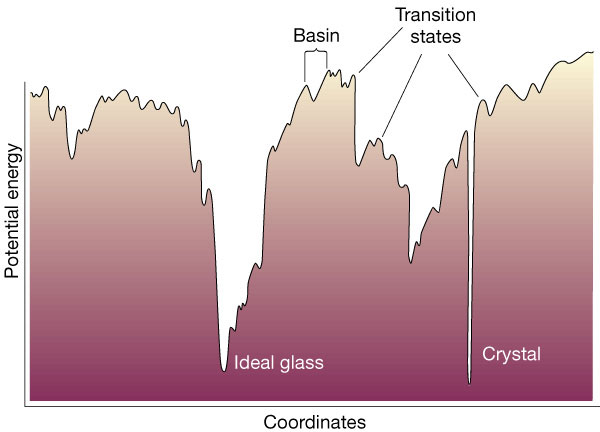
\includegraphics[width=.8\linewidth] {landscape.jpg}
	\caption{The two dimensional representation of an energy landscape for an idealized glass-forming system provided by Debenedetti and Stillinger \cite{Debenedetti}.}
	\label{figure:landscape}
\end{figure}

This is the glass transition and is perhaps well described again by \fig \nolinebreak \ref{figure:Transition} where the discontinuity in first order derivatives of the free energy are not present but rather a rapid yet smooth transition does occur as temperature decreases.  The nature of the glass transition—whether it constitutes a legitimate second-order phase transition or simply reflects rapid vitrification of the liquid state—could, in principle, be experimentally resolved in this context. If the transition is indeed smooth, lacking any discontinuity in higher-order derivatives, then the glass “transition” is merely a kinetic effect associated with a rapidly vitrifying liquid. However, if the smooth crossover implied by \fig \nolinebreak \ref{figure:Transition} does not accurately reflect the true behavior and instead a discrete discontinuity in slope exists, then the glass transition represents more than rapid vitrification; it would constitute a second-order transition in the Ehrenfest sense into a distinct thermodynamic state. Such measurements, however, do not readily provide the precision necessary to resolve a discontinuity of this kind conclusively. Nevertheless, there remains a compelling argument for the necessity of a second-order transition consistent with the observed thermodynamic behavior of glass-forming systems.

Assume for a moment that the glass "transition" is a purely kinetic vitrification process.  As depicted in \fig \nolinebreak \ref{figure:Transition}, upon super-cooling below the freezing point, $T_m$, enthalpy or specific volume will quickly approach a trend that tracks with that of the crystalline solid yet will remain systematically above the corresponding values of the crystal enthalpy as temperature continues to decrease. The exact values of enthalpy, specific volume, heat capacity, or many other bulk properties of the glassy material will depend on its thermal history including how rapidly it was quenched.  Extremely rapid thermal quenching may result in a much less ordered glassy system as molecules have virtually no time to seek out even relatively pronounced local minimums on the potential surface.  Slightly slower quenching may allow local order to arise thus giving bulk properties closer to that of the crystalline state.  For a first order phase transition, such as from a liquid to a crystalline solid, there is a specific well defined temperature at which this transition occurs.  It is desirable to define such a transition temperature for the glass transition as well.  One such definition is demonstrated in \fig \nolinebreak \ref{figure:Transition} as the intersection of the extrapolations of the linear trends in Enthalpy or specific volume as a function of temperature from well within the glassy state and from the supercooled liquid state.  These extrapolations are shown as dotted lines in \fig \nolinebreak \ref{figure:Transition} and their intersections marked as vertical dashed lines corresponding to the characteristic transition temperatures, $T_S$ and $T_R$, for a glass-forming system undergoing slow and rapid thermal quenching, respectively.  These points of intersection clearly cannot suffice as a definition for the glass transition temperature, $T_g$,  as they will inherently constitute a range of values strongly dependent upon the rate of cooling as, from an energy landscape perspective, the rate of cooling will determine to what extent the constituent molecules have time to explore the energy landscape before becoming energetically locked into a local minimum corresponding to a glassy state associated with a specific local minimum on the potential energy landscape. The more rapidly a system is quenched the more likely it is to be locked into a state that is energetically much further from the crystalline state as well as having a significantly higher residual entropy as temperature approaches absolute zero corresponding to the higher level of structural disorder.  A standard metric experimental protocol must be agreed upon if one is to define a singular glass transition temperature, $T_g$.  The most common method of defining $T_g$, at least at atmospheric pressure, has been \via calorimetric measurements which directly probe the heat capacity of the liquid as temperature is scanned at a controlled, generally agreed upon rate through the glass transition\textemdash typically ten Kelvin per minute.  At these rates a value of $T_g$ is found consistently to correspond to viscosities on the order of $10^{13}$ poise or an $\alpha-$relaxation time on the order of $100$ seconds \nolinebreak \cite{Stebbins}.  The temperatures associated with these viscosities or characteristic structural relaxation times have been generally accepted as the standard definition of the glass transition temperatures, $T_g$, throughout the literature and are those to which this work will conform.  Further details of calorimetric methods will not be  described here as these methods do not prove practical at very high pressures and were not implemented to obtain any of the data appearing in this work.  However, this thermodynamic description of the glass transition remains pertinent as it illustrates, quite effectively, one argument for the glass transition being a second order phase transition, as opposed to a purely kinematic process of rapid vitrification as will now be discussed.  

The curve labeled "Slow Quenching" in \fig \nolinebreak \ref{figure:Transition} is not, in any strict sense, a limiting case for a given glass-forming material; in principle, one may always cool more slowly. In practice, spontaneous nucleation events often induce crystallization in supercooled liquids, as observed in systems such as propylene carbonate and salol \nolinebreak \cite{Szklarz}. Similar spontaneous crystallization has also been observed in our laboratory in super-pressed salol under high-pressure conditions, where a crystalline front advanced gradually across the sample on timescales of days. However, for strong glass-formers, bulk crystallization can be suppressed even under extremely slow cooling rates.

Under such conditions, one may instead envision the formation of increasingly large locally ordered domains distributed throughout the material. These domains can progressively restrict the mobility of neighboring regions, ultimately arresting long-range structural rearrangement and producing a glassy state. The microscopic mechanisms that frustrate large-scale crystallization remain an active area of investigation \nolinebreak \cite{Shintani}.

If cooling could proceed arbitrarily slowly while still avoiding macroscopic crystallization, the bulk thermodynamic properties would be expected to approach those of the crystalline state. Extrapolation of the linear trend shown in \fig \nolinebreak \ref{figure:Transition} would then imply that the enthalpy or specific volume of the liquid could fall below that of the crystal. Such behavior would correspond to a state possessing lower entropy than the crystalline phase—an outcome known as the Kauzmann paradox \nolinebreak \cite{Kauzmann}. 

Because this scenario is thermodynamically untenable, the approach to the crystalline state must either remain asymptotic or be interrupted by a phase transition. Gibbs and DiMarzio proposed that a true second-order Ehrenfest transition could occur at the Kauzmann temperature, $T_K$, thereby resolving the paradox \nolinebreak \cite{GibbsandDiMarzio,Gibbs2}. Experimentally, however, spontaneous crystallization typically intervenes before $T_K$ can be reached, preventing direct verification of this proposal.

The argument outlined above highlights a long-standing temptation within the glass literature\textemdash namely, to interpret the apparent approach toward the Kauzmann temperature as evidence for an underlying thermodynamic phase transition. In many theoretical treatments, this transition is hypothesized to occur either at an extrapolated temperature such as $T_K$ or, in some frameworks, at a temperature above $T_g$ that would mark the onset of distinct glassy order. Mean-field and random first-order transition models, for example, predict such behavior under certain assumptions. Moreover, in disordered systems such as spin glasses, genuine thermodynamic phase transitions are well established. The situation for structural glasses, however, remains less definitive. At present, the experimental evidence does not conclusively establish whether the structural glass transition\textemdash at $T_g$, above it, or at any extrapolated temperature such as $T_K$\textemdash corresponds to a true thermodynamic phase transition.

The persistence of the higher-order interpretation stems in part from an extrapolative paradox whose logical structure bears resemblance to Zeno’s famous paradox of motion. In Zeno’s construction, a traveler attempting to reach a wall must first traverse half the distance, then half of the remaining distance, and so on \emph{ad infinitum}. Because this reasoning generates an infinite sequence of steps, it appears to forbid arrival. The flaw, of course, lies not in the subdivision of space, but in neglecting the dynamics of the process: at finite velocity, each successive interval requires half the time of the previous one, and the total traversal time forms a convergent geometric series. Once the temporal structure is properly accounted for, the paradox dissolves.

The Kauzmann paradox may be viewed as an inverted analogue of this reasoning. If one assumes that a supercooled liquid can be cooled arbitrarily slowly while remaining in thermodynamic equilibrium down to some limiting temperature, then extrapolation suggests a thermodynamic inconsistency\textemdash the entropy of the liquid falling below that of the crystal. The tension arises not from the mathematics of extrapolation, but from extending equilibrium assumptions into a regime where kinetic arrest may intervene. Introducing a thermodynamic phase transition to resolve this contradiction represents one possible interpretation, and such a scenario cannot be ruled out a priori. Nevertheless, for structural glasses, no unambiguous order parameter, symmetry breaking, or universal scaling behavior has been identified that would clearly signal such a transition.

Even if a genuine thermodynamic transition were to occur at some temperature below or even modestly above $T_g$, its signatures might be sharply defined only asymptotically close to that temperature. At experimentally accessible conditions, any associated anomalies could be progressively weakened and plausibly obscured by kinetic effects or experimental limitations. This possibility helps explain the enduring appeal of the hidden-transition hypothesis.

The central difficulty, however, is not that thermodynamic anomalies are absent near the laboratory glass transition\textemdash clear changes in quantities such as the specific heat are routinely observed\textemdash but that these signatures do not uniquely compel the existence of an underlying thermodynamic phase transition. The anomalies observed at $T_g$ are broadened, rate dependent, and consistent with kinetic arrest, making it difficult to distinguish between a true thermodynamic singularity and a dynamically induced crossover. In the absence of a well-defined order parameter or predictive framework specifying its character, the higher-order interpretation remains a plausible but unverified element of the broader theoretical landscape.

In reality, as a system is cooled toward $T_K$ under conditions of equilibrium, there exist two physically viable mechanisms by which the extrapolated Kauzmann paradox is avoided long before any such crisis is reached. The first is crystallization, which becomes increasingly thermodynamically favorable as temperature is lowered below the melting point, owing to the growing free-energy difference between the crystalline and supercooled liquid states. In principle, this enhanced thermodynamic driving force may reduce nucleation barriers and permit crystallization through pathways that do not rely exclusively on energetically activated bond breaking. In particular, entropically driven rearrangements along nearly equipotential directions of the potential-energy landscape may allow for limited structural reorganization even as thermal activation becomes suppressed.

However, the kinetic accessibility of such crystallization pathways generally diminishes as temperature is further reduced. As cooperative domain sizes grow and structural relaxation becomes increasingly collective, rearrangements require the correlated motion of ever larger regions of the material, while the available thermal energy necessary to facilitate bond breaking and large-scale reorganization is progressively denied. Under these conditions, both energetically activated and entropically driven pathways to crystallization become increasingly constrained, rendering bulk crystallization dynamically improbable despite its thermodynamic favorability.

The second, and more likely, mechanism by which the paradox is avoided is the loss of equilibrium itself. Structural relaxation time grows rapidly upon cooling, the system inevitably falls out of equilibrium at a temperature $T_g > T_K$, thereby locking in configurational entropy without inducing any thermodynamic singularity. This departure from equilibrium may occur arbitrarily sharply and at temperatures arbitrarily close to $T_K$, while remaining fully continuous in all experimentally accessible thermodynamic quantities.

The oft-invoked assertion that one may always quench more slowly, and thus asymptotically approach equilibrium down to $T_K$, is therefore no more compelling than Zeno’s conclusion that the wall can never be reached. In the limit of infinitesimal cooling rates, the time required to reach $T_K$ diverges. One does not reach $T_K$ within experimental timescales, nor within geological timescales, nor within the lifetime of the universe. 

The resolution lies not in postulating a hidden thermodynamic transition, but in recognizing the loss of ergodicity discussed previously. As relaxation times grow and eventually exceed accessible timescales, the system falls out of equilibrium and can no longer explore phase space in a manner consistent with equilibrium thermodynamics. The apparent paradox arises from extending equilibrium reasoning into a regime where ergodicity has effectively broken down.

In this sense, the Kauzmann construction does not by itself compel the existence of a higher-order thermodynamic phase transition. Rather, it highlights the limitations of equilibrium extrapolation in systems whose relaxation times diverge.


\section{Probes of Glassy Dynamics} \label{sec:probes}

In this section, we will introduce and briefly discuss a selection of widely used experimental techniques—such as depolarized photon correlation spectroscopy (DPCS), depolarized Brillouin light scattering (DBLS), and dielectric spectroscopy (DS)—that provide complementary insight into the molecular dynamics underpinning the glass transition.

Although the calorimetric method of defining the glass transition temperature, $T_g$, as described above is theoretically compelling and remains the standard at atmospheric pressure, it does require a large amount of data, taken with tight experimental control of the cooling/heating rates, in order to arrive at reproducible values for the glass transition temperature, $T_g$. As mentioned above, it is experimentally advantageous to define the glass transition temperature in terms of viscosity or, equivalently, the characteristic structural relaxation time.  The characteristic timescales on which molecular dynamics evolve in a glass-forming system vary from on the order of picoseconds for very high-temperatures or in low pressure environments, to thousands of seconds at low temperatures or in high pressure environments. Due to this extreme dynamic range, a single experimental probe for tracking these molecular dynamics will likely never exist; and in fact, experimental gaps within the literature typically exist for dynamic data on any given glass-forming system.  Be that as it may, with the aid of a proper mathematical model and the implementation of several different experimental probes, each within their applicable dynamic window, excellent descriptions of these dynamics can be ascertained over exceedingly large dynamic ranges encompassing the glass transition for many materials.  

At this point, the astute reader may be asking a simple question: what are "these dynamics"?   Specifically, the study of the glass transition relies on experimental probes capable of tracking changes in molecular or atomic locations and orientations.  Some may accomplish this directly, perhaps \via some scattering mechanism that tracks thermal diffusion, or more indirectly \via tracking changes to thermodynamic bulk properties such as viscosity which arises as a direct consequence of said diffusion. This work will exclusively  focus on probes of viscosity, $\eta$, and the characteristic structural $\alpha$-relaxation time, $\tau_{\alpha}$.  These two bulk properties are intrinsically related \via the Maxwell relation, which states that for small deformations or applied strain,

\begin{equation}
	\tau_{\alpha} = \frac{\eta}{G_{\infty}},
	\label{eq:MaxwellRelation}
\end{equation}

\noindent where $G_{\infty}$ is the high-frequency shear modulus.  \fig \nolinebreak \ref{figure:MaxwellRelaxation} illustrates how the stress resulting from an adiabatically applied strain relaxes over time due to viscous flow of the bulk material. 

\pgfplotsset{table/search path={Chapters/Background/Figures},}
\begin{figure}[!htbp]
	\centering
	
	\begin{tikzpicture} 
		\begin{axis}[
			height=.5\textwidth,
			width=.75\textwidth,
			ylabel={Normalized Modulus $\left(\frac{G\left(t\right)}{G_\infty}\right)$},
			xlabel={Normalized Time $\left(\nicefrac{t}{\tau}\right)$},
			xmin=0, xmax=3,
			ymin=0, ymax=1,
			ymajorgrids=false,
			grid style=dashed,
			]	
			\addplot table [mark=none,x=time, y=stress, col sep=comma] {MaxwellRelation.csv};	
		\end{axis} 
	\end{tikzpicture}
	
	\caption{An idealized stress relaxation response following the rapid imposition of a small step strain, $\epsilon_0$, in the linear viscoelastic regime. The stress, $\sigma\!\left(t\right)$, is normalized by $G_\infty\epsilon_0$, where $G_\infty$ is the instantaneous shear modulus. The characteristic relaxation time over which viscous flow mediates mechanical stress relaxation is $\tau=\nicefrac{\eta}{G_\infty}$.}  
	\label{figure:MaxwellRelaxation}
\end{figure}


However direct measurements of structural relaxation and viscosity are certainly not the only window into glassy dynamics. \fig \nolinebreak \ref{figure:Transition} illustrates a classical dilatometric determination of the glass transition temperature, in which the underlying molecular dynamics are not directly probed. Instead, the specific volume is monitored as a function of temperature. In calorimetric measurements, the corresponding signature appears in the temperature dependence of the heat capacity, $C_p$. Both approaches track bulk thermodynamic quantities that emerge from the collective molecular dynamics of the system.  \fig \nolinebreak \ref{GlassCorrComp}, though not comprised of actual data, is representative of that which has been obtained \via direct structural probes such as neutron scattering.  However neutron scattering has provided more than just structural snapshots.  Though it will not be discussed in great detail here, as it is not directly relevant to the data presented in this work, inelastic and quasielastic neutron scattering have also served as probes of molecular dynamics in glassy systems. These techniques are sensitive to motions on picosecond to nanosecond timescales, enabling the study of vibrational excitations and fast relaxational processes \nolinebreak \cite{SinclairRN, Tolle, Jurkiewicz}.

\begin{figure}[!htbp]
	\centering
	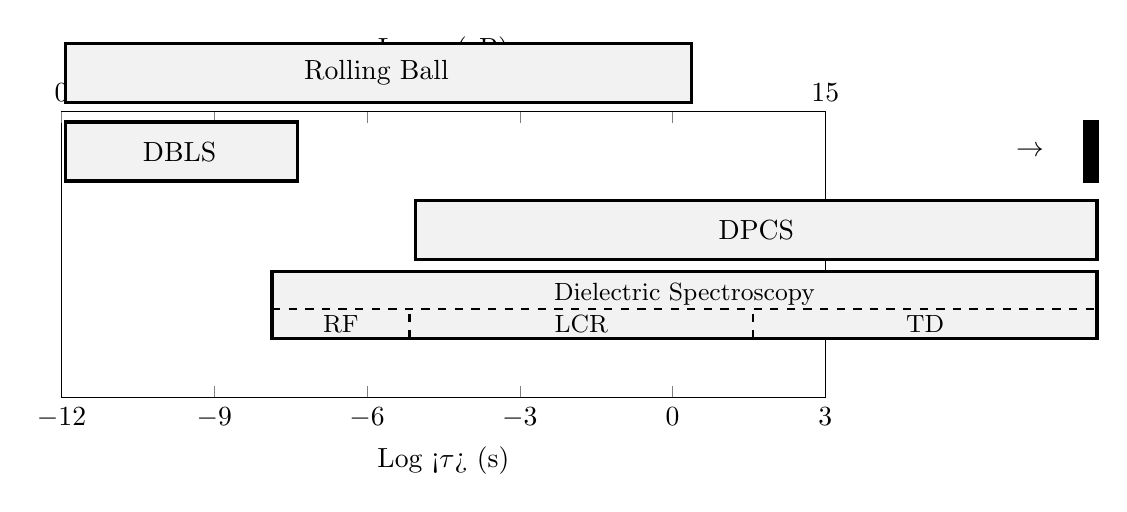
\begin{tikzpicture} 
		
		\begin{axis}[
			width=0.8\textwidth,
			height=0.3\textwidth,
			xlabel={Log <$\tau$> (s)},
			scale only axis,
			xmin=-12,xmax=3,
			xtick distance = 3,
			ymin=0,ymax=1,
			ytick=\empty,
			axis y line*=left,
			axis x line*=bottom]
			\addplot[]{-10}; %Just here to force the axis to print
		\end{axis}
		
		\begin{axis}[
			width=0.8\textwidth,
			height=0.3\textwidth,
			scale only axis,
			xmin=0,xmax=15,xtick={0,3,6,9,12,15},
			ymin=0,ymax=1,
			xtick distance = 5,
			ytick=\empty,
			domain=0:15,
			axis y line*=right,
			axis x line*=top,
			xlabel={Log $\eta$ (cP)}]
			\addplot[]{-10}; %Just here to force the axis to print
		\end{axis}
		
		%Box Representation of Rolling Ball
		\filldraw[black,fill=black!5, very thick] (0.055,3.75) rectangle (8,4.5);
		
		%Box Representation of DBLS
		\filldraw[black,fill=black!5, very thick] (0.055,2.75) rectangle (3,3.5);
		
		%Box Representation of DPCS
		\filldraw[black,fill=black!5, very thick] (4.5,1.75) rectangle (13.15,2.5);
		
		%Box Representation of DS
		\filldraw[black,fill=black!5, very thick] (2.674,0.75) rectangle (13.15,1.6);
		
		%Internal dashed divisions for DS
		\draw[dashed, thick] (2.674,1.125) -- (13.15,1.125);    %horizontal divider
		\draw[dashed, thick] (4.420,0.75) -- (4.420,1.125);     %RF | LCR at log tau = -7
		\draw[dashed, thick] (8.785,0.75) -- (8.785,1.125);     %LCR | TD at log tau = -2
		
		%Box Representation of TgP
		\filldraw[black,fill=black!100, very thick] (13,2.75) rectangle (13.15,3.5);
		
		\node at (12.3,3.125) {\tgp $\rightarrow$};
		\node at (4,4.125) {Rolling Ball};
		\node at (1.5,3.125) {DBLS};
		\node at (8.825,2.125) {DPCS};
		
		%DS labels
		\node[font=\small] at (7.912,1.3125) {Dielectric Spectroscopy};
		\node[font=\small] at (3.547,0.9375) {RF};
		\node[font=\small] at (6.6025,0.9375) {LCR};
		\node[font=\small] at (10.9675,0.9375) {TD};
		
	\end{tikzpicture}
	\caption{Accessible dynamic ranges for various probes of viscosity $\eta$ and structural relaxation time $\tau_\alpha$. Rolling Ball: rolling-ball viscometry (probe of $\eta$); DBLS: depolarized Brillouin light scattering; DPCS: depolarized photon correlation spectroscopy; DS: dielectric loss spectroscopy, shown as a composite of experimental regimes (dashed divisions): radio-frequency (RF), impedance/LCR, and time-domain (TD) measurements; \tgp: technique described in \sect\nolinebreak \ref{sec:IGPintro}.}
	\label{figure:Probes}
\end{figure}

The experimental probes referenced or implemented in this work are summarized in \fig \nolinebreak \ref{figure:Probes}. These include DPCS, DBLS, rolling ball viscometry, \tgp analysis, and DS. The physical mechanism behind each of these probes will be described briefly below as well as their dynamic windows and other limitations to their applicability pertinent to this work.  These descriptions will be kept intentionally brief as an entire dissertation could easily be written on any one of these probes alone, and indeed, \chap\nolinebreak \ref{chap:Glycerol} is in effect a reanalysis of one such dissertation outlining a means of extending a previously existing probe, rolling ball viscometry, into a diamond anvil cell allowing for viscosity measurements at higher pressures.\cite{CookThesis}  Following this, \chap\nolinebreak \ref{chap:PCS} will provide a similar extension, this time of photon correlation spectroscopy, into the diamond anvil cell.  Significantly more detail regarding these specific probes will be provided in their respective chapters.

\subsection{Depolarized Brillouin Light Scattering (DBLS)}
Electromagnetic interactions with matter lie at the heart of most experimental probes of structure and dynamics. Notable exceptions include ultrasonic techniques and neutron scattering, which rely on mechanical or nuclear interactions rather than electromagnetic coupling. Nevertheless, even neutron scattering possesses an electromagnetic aspect: the neutron’s appreciable magnetic moment renders it uniquely sensitive to ordered magnetic structures, such as spin fluctuations in superconducting materials \cite{Zaliznyak}. 

Light scattering methods probe how condensed matter responds to incident electromagnetic radiation, giving rise to a scattered field that carries information about the structure and dynamics of the bulk material. A generalized schematic for a light scattering experiment is shown in \fig \nolinebreak \ref{figure:SimpleDLS}. Polarized monochromatic laser light is collimated or focused through a sample volume, and a fraction of this light is scattered, collected, and directed onto a suitable spectral analyzer.

In the experiments presented in this dissertation, an intracavity etalon was employed to ensure single-mode laser operation with a spectral width of approximately $10~\si{\mega\hertz}$, as required for high-resolution Brillouin measurements. It is worth noting that other light scattering techniques, such as Raman scattering, commonly utilize multi-mode lasers with linewidths on the order of $\sim\si{\giga\hertz}$—still only about one part in $10^6$ of the optical carrier frequency. The scattered light in this work is analyzed using either a triple-pass tandem Fabry-P\'erot interferometer (DBLS) or a photon correlation spectrometer (DPCS).


\begin{figure}[!htbp]
	\centering
	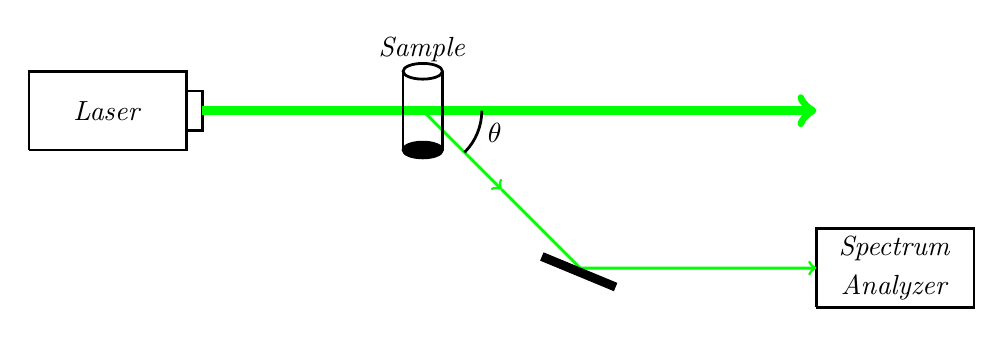
\begin{tikzpicture}
	%Laser
	\draw[line width=1pt] (0,0)--(2,0)--(2,1)--(0,1)--(0,0);
	\draw[line width=1pt] (2,.25)--(2.2,.25)--(2.2,.75)--(2,.75);
	\node[] at (1,.5) () {\textit{Laser}};
	
	%PMT
	\draw[line width=1pt] (10,-2)--(12,-2)--(12,-1)--(10,-1)--(10,-2);
	\node[] at (11,-1.25) () {\textit{Spectrum}};
	\node[] at (11,-1.75) () {\textit{Analyzer}};
	
	%Beams
	\draw[line width=3pt,color=green,->] (2.2,.5)--(10,.5);
	\draw[line width=1pt,color=green,->] (5,.5)--(6,-.5);
	\draw[line width=1pt,color=green,->] (6,-.5)--(7,-1.5)--(10,-1.5);
	\draw[line width=1pt] (5.75,.5) arc (0:-45:.75) node[midway,anchor=west] {$\theta$};
	
	%splitters
	\node[] at (7,-1.5) (c) {};
	\draw[rotate around={-22.5:(c)},fill=black] (7.5,-1.5) rectangle (6.5,-1.6);
	
	%Scatter Volume
	\node[anchor=south] at (5,1) () {\textit{Sample}};
	\node[] at (5,.5) (d) {}; %scatter volume center
	\draw[line width=1pt,fill=black] (5,0) ellipse (.25 and .1);
	\draw[line width=1pt] (5,1) ellipse (.25 and .1);
	\draw[line width=1pt] (5.25,0)--(5.25,1);
	\draw[line width=1pt] (4.75,0)--(4.75,1);
	
	\end{tikzpicture}
	\caption{A simple forward scattering DBLS experimental design in which light from a monochromatic source, such as a single mode locked AR\textsuperscript{+} laser, is scattered from a sample and collected at a known angle.  The collected light is then directed into a spectrum analyzer, such as a triple pass tandem Fabry-P\'erot interferometer.}\label{figure:SimpleDLS}
\end{figure}

A light source with exceedingly narrow spectral width is necessary for DBLS, as this probe resolves very small frequency shifts in the scattered light arising from dynamic processes within the sample. These processes will be described in more detail in \sect \nolinebreak \ref{sec:TheScatteredField} and \nolinebreak \ref{sec:SpectrumOfSimpleFluid}; for now, it suffices to note that light is scattered whenever there is a local temporal or spatial variation in the dielectric susceptibility of the medium. Such variations may arise from density fluctuations, induced dipoles, or orientational dynamics—anything that alters how the charges within the material respond to an applied electromagnetic field. If the susceptibility variation is purely spatial and static—for example, in a material with frozen-in density inhomogeneities—the scattered field retains the frequency of the incident beam, giving rise to elastic (Rayleigh) scattering. In fluids, however, density fluctuations are inherently time dependent. Any temporal modulation of the dielectric susceptibility must therefore produce a corresponding distribution of frequencies in the scattered field. Even crystalline solids exhibit such time-dependent fluctuations due to lattice vibrations. Longitudinal and transverse acoustic modes, as well as higher-frequency optical phonons, appear as frequency-shifted features in the scattered spectrum.

Depolarized Brillouin Light Scattering (DBLS), as implemented in this work, refers to the spectral analysis of depolarized scattered light using a high-resolution Fabry-P\'erot interferometer. Brillouin scattering arises from the interaction of light with thermally excited acoustic modes in the material—long-wavelength density fluctuations corresponding to small wavevector phonons in the GHz frequency regime. This distinguishes Brillouin scattering from Raman spectroscopy, which probes optical phonons or intramolecular vibrational modes at much higher (THz) frequencies and whose larger energy shifts are typically resolved using grating-based spectrometers.

In glass-forming liquids, the depolarized Brillouin spectrum contains not only acoustic sidebands but also a central quasielastic component. It is this central quasielastic feature, arising from time-dependent fluctuations in the anisotropic part of the dielectric susceptibility, that is of primary interest in the present work. This spectral component reflects structural relaxation processes within the bulk material and provides a direct probe of the $\alpha$-relaxation over a dynamic window approximately bounded by 
\[
10^{-12}\;\si{\second} \lesssim \tau_\alpha \lesssim 10^{-9}\;\si{\second},
\]
as shown in \fig \nolinebreak \ref{figure:Probes}.

While analysis of the linewidths of longitudinal acoustic (LA) Brillouin modes can provide access to viscoelastic damping and relaxation phenomena over a broader dynamic range \cite{Heiman}, such approaches probe relaxation indirectly through mechanical response functions. In contrast, the DBLS measurements discussed here focus specifically on the quasielastic depolarized spectrum as a more direct probe of structural $\alpha$-relaxation.

It is important to distinguish this spectrally resolved DBLS method from photon correlation spectroscopy (DPCS), which also probes $\alpha$-relaxation but does so through analysis of temporal fluctuations in scattered intensity rather than through frequency-domain spectral analysis. The two techniques therefore access distinct dynamic windows and rely on fundamentally different measurement formalisms.

\subsection{Depolarized Photon Correlation Spectroscopy (DPCS)} \label{sec:PCSintro}

Depolarized photon correlation spectroscopy (DPCS) is a light scattering technique, similar to DBLS described above, yet performed in the time domain. Both methods provide access to the $\alpha$-structural relaxation dynamics within a glass-forming liquid, however, they cover vastly different dynamic ranges. Whereas DBLS lends itself to probing very fast relaxations, on the order of tens to thousands of picoseconds, DPCS is generally applicable in the slow to intermediate dynamic regime, probing characteristic relaxation times ranging from tens of nanoseconds to thousands of seconds. A typical experimental setup for DPCS is shown in \fig \nolinebreak \ref{figure:SimpleDLS} \textemdash differing from DBLS only in the form of analyzer implemented. In fact, data taken for both DBLS and DPCS, analyzed in \chap \nolinebreak \ref{chap:PCS}, were all acquired on a single experimental setup in which a flip mirror allowed the collected scattered light from a sample to be directed either into a tandem triple-pass Fabry–Perot interferometer for frequency analysis or, alternatively, into a digital autocorrelator for temporal analysis.

There are two general experimental domains relevant to PCS\textemdash heterodyne and homodyne autocorrelation. It is important to define these terms here as there is some discrepancy within the literature regarding their use.  For the purposes of this work, homodyne PCS involves temporal correlation analysis of light scattered from a sample, where great care is taken to ensure that the detected signal arises solely from spontaneous density fluctuations within the material. Particular attention is given to minimizing parasitic elastic scattering and specular reflections from dust, cell windows, culets, or table surfaces, which could act as a coherent local oscillator and introduce heterodyne contributions to the measured correlation function.  The intensity of this scattered light will fluctuate as a result of any temporal dependency associated with these dynamic processes.  As such, this experimental arrangement is often referred to as ``self-beating,'' a designation that only becomes meaningful when contrasted with the alternative PCS configuration\textemdash heterodyne detection.

In a heterodyne experimental arrangement, such as is represented in \fig \nolinebreak \ref{figure:simpleHeterodyne}, a fraction of the source laser is split off before it is passed through the scattering sample and then re-mixed before being directed onto the detector for autocorrelation. In this arrangement, the fluctuations in detected intensity do not arise from the total number of scattering events, but rather from a shift in phase between light arising from scattering events and that of the local oscillator\textemdash a portion of the laser being mixed in providing a phase reference for the scattered light to beat against.  Below is shown one possible heterodyne experimental arrangement.  It is also common simply to collect light from the sample such that the specular reflection from the container can itself provide a local oscillator.  All that is required to operate within a heterodyne regime is that the local oscillator intensity be significantly greater than that of the light scattered from the sample.   Conversely, if one wishes to operate in a homodyne regime, one must ensure that any specular reflections or contributions from static scattering are negligible compared to the light scattered by the dynamic processes of interest within the sample. This often requires significant spatial filtering as well as exceedingly pure samples and clean experimental environments.

\begin{figure}[!htbp]
	\centering
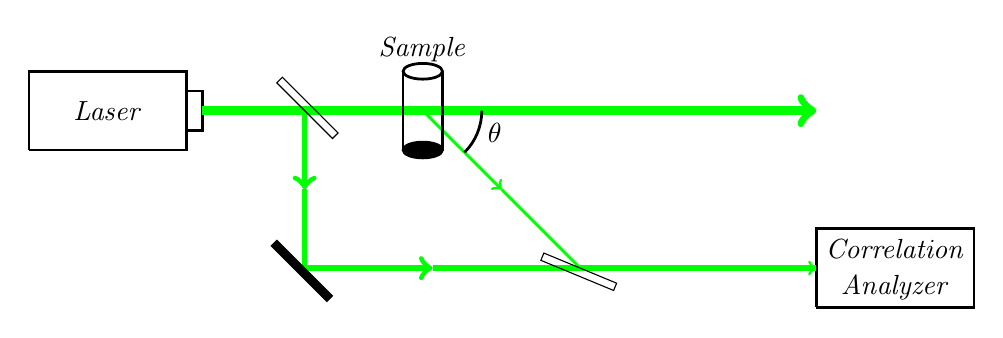
\begin{tikzpicture}
	%Laser
	\draw[line width=1pt] (0,0)--(2,0)--(2,1)--(0,1)--(0,0);
	\draw[line width=1pt] (2,.25)--(2.2,.25)--(2.2,.75)--(2,.75);
	\node[] at (1,.5) () {\textit{Laser}};
	
	%PMT
	\draw[line width=1pt] (10,-2)--(12,-2)--(12,-1)--(10,-1)--(10,-2);
	\node[] at (11,-1.25) () {\textit{Correlation}};
	\node[] at (11,-1.75) () {\textit{Analyzer}};
	
	%Beams
	\draw[line width=3pt,color=green,->] (2.2,.5)--(10,.5);
	\draw[line width=1pt,color=green,->] (5,.5)--(6,-.5);
	\draw[line width=1pt,color=green,->] (6,-.5)--(7,-1.5)--(10,-1.5);
	\draw[line width=1pt] (5.75,.5) arc (0:-45:.75) node[midway,anchor=west] {$\theta$};
	\draw[line width=2pt,color=green,->] (3.5,.5)--(3.5,-.5);
	\draw[line width=2pt,color=green] (3.5,-.5)--(3.5,-1.5);
	\draw[line width=2pt,color=green,->] (3.5,-1.5)--(5.125,-1.5);
	\draw[line width=2pt,color=green] (5.125,-1.5)--(10,-1.5);
	
	%splitters
	\node[] at (3.5,.5) (a) {}; %splitter center
	\draw[rotate around={-45:(a)}] (3,.5) rectangle (4,.6);
	\node[] at (3.5,-1.5) (b) {}; %splitter center
	\draw[rotate around={-45:(b)},fill=black] (3,-1.5) rectangle (4,-1.6);
	\node[] at (7,-1.5) (c) {};
	\draw[rotate around={-22.5:(c)}] (7.5,-1.5) rectangle (6.5,-1.6);
	
	%Scatter Volume
	\node[anchor=south] at (5,1) () {\textit{Sample}};
	\node[] at (5,.5) (d) {}; %scatter volume center
	\draw[line width=1pt,fill=black] (5,0) ellipse (.25 and .1);
	\draw[line width=1pt] (5,1) ellipse (.25 and .1);
	\draw[line width=1pt] (5.25,0)--(5.25,1);
	\draw[line width=1pt] (4.75,0)--(4.75,1);

\end{tikzpicture}
\caption{Heterodyne experimental arrangement for PCS.  A local oscillator is mixed with the scattered signal before being redirected onto the photomultiplier or other detector.}
\label{figure:simpleHeterodyne}
\end{figure}

In both experimental arrangements the intensity fluctuations at the detector are due to the same fluctuations in the local density or dielectric constant within the scattering volume in the sample, however, the two methods measure different correlation functions of these fluctuations.  Thus, proper analysis of resulting data requires that one be firmly within one or the other experimental domain.  It is generally very undesirable to be within an intermediate homodyne/heterodyne scenario.  If a homodyne experiment is desired one must often take great care to assure that only light arising from the scattering events of interest are collected.  Dust and contaminates, both within the sample and on the sample container, or even undesired specular reflections may give rise to undesired heterodyne components which may make proper data analysis challenging or even impossible.  These concerns are not always easily mitigated, and great care is required to identify the regime in which one is operating, as will be discussed in \sect \nolinebreak \ref{sec:HomoHeto}, where a method for extending PCS to high-pressure is described in detail.


\subsection{Rolling Ball Viscometry} \label{sec:rolling_ball}

Rolling or falling Ball viscometry provides a means of direct mechanical measurement of viscosity.  Many different types of high pressure vicometers and their range of application are described in more detail by Cook, Herbst, and King\cite{Cook}.  These methods generally implement a spherical ball as it moves through a viscous fluid under the influence of gravity or other forces.  Placing this ball within a diamond anvil cell allows access to very high pressures however the viscosities that can be measured are obviously limited to those low enough for a macroscopic ball to progress through the material during the course of a reasonable experimental timescale.  In practice this means that rolling and falling ball viscometry in a diamond anvil cell is limited to approximately $10^7$ cP\textemdash eight orders of magnitude away from the glass transition.  In the work previously cited, Cook \etal managed to extend this viscosity range an additional two and a half orders of magnitude, up to approximately $10^{9}$ cP, \via placing the diamond anvil cell viscometer onto a centrifuge which greatly increases the g-forces driving the ball through the fluid\cite{Cook}.  However this still limits the probe to a viscosity range many orders of magnitude away from the glass transition.

Though this probe cannot provide measurements in the vicinity of the glass transition it does, as shown in \fig \nolinebreak \ref{figure:Probes}, provide access to a very large dynamic range of viscosities\textemdash up to nine orders of magnitude.  There are some experimental concerns even within its range of application.  Specifically, rolling ball viscometry relies on a correction, or ``wall factor,'' that accounts for dissipative losses as the ball rolls down the diamond surface within the cell.  This correction factor is assumed to be constant as experimental variables such as pressure and temperature are changed.  It is also generally assumed that the probe ball is rolling down the diamond cutlet without slipping.  It is very difficult, if not impossible, to directly verify the degree to which these assumptions hold over the entire range of experimental parameters.  However this work will show that data for the glass former glycerol obtained by Cook \etal \via rolling ball viscometry appears to be reasonably consistent over its applicable range with data taken \via other probes and non-related methods.

\subsection{\tgp} \label{sec:IGPintro}

The \tgp process is a very straight forward means of measuring the isochronal curve of the glass transition temperature $T_{g}$ as a function of Pressure.  A liquid is loaded into a diamond anvil cell and brought to a temperature and pressure such that it is well within the solid glass phase.  It has been found advantageous to pre-indent the gasket, which hardens it, thus making higher pressures more achievable.  Two or more rubies are arranged throughout the sample as shown in the far left DAC in \fig \nolinebreak \ref{figure:tgpgrade}.  A pressure gradient is then applied to the DAC \via asymmetric application of force as indicated by the dashed Isobaric Lines. 
\begin{figure}[!htbp]
	\centering
	\includegraphics[width=0.8\textwidth]{gradient.jpg}
	\caption{Pressure gradients established within a diamond anvil cell decrease as temperature increases and the system approaches the glass transition from the glassy state, ultimately attaining hydrostatic conditions. This figure is reproduced from Ref.~\cite{RansomPRL}.}
	\label{figure:tgpgrade}
\end{figure}
Temperature is then increased incrementally, typically in 5 to 10 degree steps initially and then smaller steps as the glass transition is approached as evident \via the pressure gradients giving way to hydrostatic conditions above $T_{g}$.  At each temperature, pressure is measured from a consistent  location on each ruby to again check for pressure gradients.  Temperature is then increased to a new set point and a small set time is allowed for the sample to reestablish thermal equilibrium.  A means of determining the approximate temperature at which the gradients dissolve and the material transitions into a liquid have been developed previously and described in Ref. \nolinebreak \cite{RansomPRL,Ransom}.  The values obtained for the glass transition temperatures as a function of pressure are fit to an Andersson-Andersson equation \cite{Andersson} provided along with data for glycerol and cumene in \app \nolinebreak  \ref{app:GlycerolIGP} and \nolinebreak \ref{app:CumeneIGP} respectively. The automation of this process will increase its efficacy in the future and may even allow it to provide more than a single isochronal curve near and around the glass transition.  


\subsection{Dielectric Loss Spectrometry} \label{sec:FRAintro}

Frequency Response Analysis encompasses various methods capable of measuring molecular dynamics over an exceptionally broad dynamic range. Among these, Dielectric Spectroscopy (DS) is particularly important and will be extensively discussed in this dissertation. DS takes advantage of molecular dipole moments, which either inherently exist or are induced by an applied oscillating electric field.

As molecular orientations within the glass-forming liquid respond to an applied external field, dielectric spectroscopy (DS) measures both the real and imaginary components of the complex dielectric constant. When the frequency of the applied field is systematically swept—from fractions of a hertz to several gigahertz—the imaginary component plotted as a function of frequency forms the dielectric loss spectrum. Peaks in this loss spectrum correspond directly to molecular relaxation processes occurring within the sample. 

Alternatively, DS measurements may be performed at fixed frequency while varying temperature or pressure, with both components of the dielectric response recorded as functions of $T$ or $P$. In either protocol, the rate at which frequency, temperature, or pressure is varied plays an important role in determining the apparent relaxation behavior. By monitoring how the positions of loss maxima evolve under controlled thermodynamic conditions, researchers gain access to molecular dynamics such as the structural relaxation time ($\tau_{\alpha}$), as well as faster secondary processes, commonly referred to as $\beta$-relaxations.

However, dielectric spectroscopy provides considerably more information than merely the characteristic structural relaxation times inferred from dielectric loss peaks. Both the real and imaginary components of the complex dielectric constant contain dynamical information. When analyzed together, these components may be represented in the complex plane to form characteristic Cole--Cole or Cole--Davidson plots \cite{Davidson}. Such representations facilitate visualization of relaxation behavior and, when combined with appropriate empirical response functions, enable extraction of additional parameters. Among these is the stretching exponent $\beta$, which reflects the breadth of the underlying distribution of relaxation times and the degree of dynamical heterogeneity within the glass-forming liquid. Representative examples illustrating both Debye-like and stretched-exponential behavior are presented in \chap \nolinebreak \ref{chap:Glycerol} (see, for example, \fig \nolinebreak \ref{figure:glcyerolcolecole}).

Given its capability to provide a wide array of parameters and its extensive dynamic range, dielectric spectroscopy is one of the most powerful and widely implemented experimental methods in glass transition research. Indeed, due to its comprehensive coverage of both structural and secondary relaxations, DS serves as an indispensable tool for studying the complex molecular dynamics of glass-forming liquids, a role this dissertation will explore further.
